%!TEX TS-program = xelatex
\documentclass[]{friggeri-cv}
\usepackage{afterpage}
\usepackage{hyperref}
\usepackage{color}
\usepackage{xcolor}
\hypersetup{
    pdftitle={},
    pdfauthor={},
    pdfsubject={},
    pdfkeywords={},
    colorlinks=false,       % no lik border color
   allbordercolors=white    % white border color for all
}
\RequirePackage{xcolor}
\definecolor{pblue}{HTML}{0395DE}

\usepackage{enumitem}

\begin{document}
\header{Victor M.}{Mendiola-Lau}{Científico de la Computación, Investigador e Ingeniero de Software}
      
% Fake text to add separator      
\fcolorbox{white}{gray}{\parbox{\dimexpr\textwidth-2\fboxsep-2\fboxrule}{%
.....
}}

% In the aside, each new line forces a line break
\begin{aside}
  \section{Dirección}
    Ayuntamiento 7375, 
    La Habana, Cuba
    ~
    ~
    ~
  \section{Teléfono}
    (+53) 5 413 2909 (cell)
  	(+53) 7 873 0125 (home)
    ~
    ~
    ~
  \section{Correo}
    \href{mailto:ryuzakyl@gmail.com}{\textbf{ryuzakyl@}gmail.com}
	~
	~    
    ~
  \section{Perfiles web}
    \href{https://github.com/ryuzakyl}{{\scriptsize github.com/ryuzakyl}}
    \href{https://independent.academia.edu/VictorMendiolaLau}{{\scriptsize academia.edu/VictorMendiolaLau}}
    \href{https://www.linkedin.com/in/VictorMendiolaLau}{{\scriptsize linkedin.com/in/VictorMendiolaLau}}
	\href{https://www.researchgate.net/profile/Victor_Mendiola-Lau}{{\scriptsize researchgate.net/Victor\char`_Mendiola-Lau}}
    ~
    ~
    ~
  \section{Habilidades personales}
    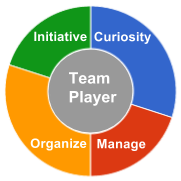
\includegraphics[scale=0.62]{img/personal.png}
    ~
%    ~
%  \section{Programming}
%    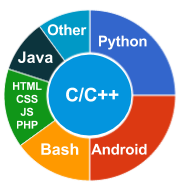
\includegraphics[scale=0.62]{img/programming.png}
%    ~
\end{aside}

\section{Ingeniería de Software}
\begin{entrylist}
  \entry
    {09/18 - Now}
    {Ingeniero de Software}
    {Kitsune Technologies, Tennessee, EUA}   
    {Amplia gama de responsabilidades, incluyendo Análisis de Datos, Visión por Computadora, Desarrollo Web, implementación de servicios, etc.\\}

  \entry
    {09/17 - 11/18}
    {Desarrollador Web Full Stack}
    {}
    {Aplicaciones web como soluciones al manejo de las fuerzas de trabajo. Tecnologías: PHP, HTML, CSS3, JavaScript, jQuery, MySQL, etc.\\}
    
  \entry
    {12/17 - 02/18}
    {Desarrollador de Backend en Python/Django}
    {SBY Technologies, Florida, EUA}
    {Desarrollo de un API desde cero con autenticación mediante JWT, generación automática de reportes (.pdf, .csv), etc. También desempeñé el rol de ingeniero de DevOps y Administrador de Sistemas en Linux.\\}
    
  \entry
    {02/16 - 03/16}
    {Desarrollador de Backend en Ruby/Rails}
    {Ksabes, La Habana, Cuba}
    {Diseño e implementación propia de un API basada en Json Web Token (JWT) para la autenticación.\\}

  \entry
    {09/14 - 01/15}
    {Desarrollador de Ruby}
    {IRStrat, México D.F., México}
    {Diseño e implementación propia de un servicio concurrente y multi-hilos para consumir información de la bolsa de valores en tiempo real.\\}

  \entry
    {09/13 - 09/17}
    {Ingeniero de Software}
    {CENATAV, La Habana, Cuba}
    {Desarrollador de Aplicaciones de Escritorio Full Stack en .NET Framework, específicamente en C\#. Diseño y desarrollo eficiente de algoritmos en C/C++. Integración de aplicaciones de escritorio en .NET con bibliotecas implementadas en C/C++ mediante PInvoke.\\}    
    
\end{entrylist}

\section{Otras responsabilidades}
\begin{entrylist}
  \entry
    {11/18 - Ahora}
    {Consultor}
    {PNWA, Seattle, USA}
    {Miembro del grupo consultor Pacific NorthWest Advisors (PNWA) realizando estudios de mercado y de la informática dentro de Cuba y brindando también información única a las empresas del noroeste del Pacífico.}

\end{entrylist}

\section{Educación/Formación académica}
\begin{entrylist}
%  \entry
%    {2009 - 2012}
%    {Master's Degree in Computer Engineering}
%    {Università di Pisa, Italy}
%    {Curriculum Networking and Multimedia.\\
%    Main subjects: Network Applications, Systems Architecture and Security, Mobile Applications, Multemedia Information            Processing.\\
%    \emph{Title of the Thesis: "A Handoff Algorithm based on Link Quality Prediction for Mass Transit Wireless Mesh Networks"      .}\\
%    \emph{Relators: Prof. Enzo Mingozzi, Ing. Carlo Vallati, Prof. Luciano Lenzini.}\\}

  \entry
    {2008 - 2013}
    {B.Sc. en Ciencia de la Computación}
    {Universidad de La Habana, Cuba}
    {Título de Oro (5.13 de 5.0) en Ciencia de la Computación. Materias principales: Programación, Estructuras de Datos y Algoritmos, Teoría de la Complejidad Computacional, Matemática, Investigación Operacional, Matemática Numérica e Inteligencia Artificial.\\
    \emph{Título de la Tesis: "Reconocimiento de iris utilizando Análisis de Datos Funcionales".}}

%  \entry
%    {2004 - 2007}
%    {Bachelor Diploma}
%    {IPVCE Vladimir Ilich Lenin, Havana, Cuba}
%    {Bachelor diploma with focus on these subjects: Matematics and Computer Science.}
\end{entrylist}

\pagebreak

\section{Idiomas}
\begin{entrylist}
  \entry
    {\textbf{Español}}
    {}
    {}
    {Lengua materna}      

  \entry
    {\textbf{Inglés}}
    {}
    {}
    {Graduado \textbf{\emph{summa cum laude}} de la Escuela de Idiomas \emph{Abraham Lincoln}.}

  \entry
    {\textbf{Francés}}
    {}
    {}
    {Diploma de estudios de la Lengua Francesa (\textbf{DELF B2}).}
\end{entrylist}

\section{Certificados \& Cursos de formación}
\begin{entrylist}
  \entry
    {2014}
    {(Postgrado) Metodologías de la Investigación}
    {CENATAV, IDICT}
    {\emph{Desmitificar la investigación y los métodos de investigación. Bosquejo de los fundamentos de la investigación.}}
\end{entrylist}

\begin{entrylist}    
  \entry
    {2013}
    {(Tutorial) Fundamentos del Reconocimiento de Iris}
    {Congreso CIARP 2013}
    {\emph{Tutorial presentado por el Profesor Tieniu Tan sobre los avances y retos del Reconocimiento de Iris.}}

  \entry
    {}
    {(Tutorial) Análisis de grandes volúmenes de datos}
    {Congreso CIARP 2013}
    {\emph{Minería de datos inciertos y probabilísticos para grandes volúmenes de datos por el Profesor Jian Pei.}}
    
  \entry
    {}
    {(Licenciatura) \LaTeX}
    {Universidad de La Habana}
    {\emph{Introducción al lenguaje de descripción de documentos construido sobre \TeX.}}
\end{entrylist}
       
\begin{entrylist}
  \entry
    {2012}
    {(Postgrado) Estructuras de Datos Avanzadas}
    {Universidad de La Habana}
    {\emph{Introducción a conceptos como el Análisis amortizado, Heaps de Fibonacci, Splay Trees, etc.}}      

  \entry
    {}
    {(Licenciatura) Inteligencia de Negocios}
    {Universidad de La Habana}
    {\emph{Introducción a los conceptos fundamentales de los procesos modernos de Inteligencia de Negocios.}}

  \entry
    {}
    {(Licenciatura) Introducción a la Criptografía}
    {Universidad de La Habana}
    {\emph{Introducción a los conceptos fundamentales de la Criptografía moderna.}}
\end{entrylist}

\begin{entrylist}
  \entry
    {2011}
    {(Licenciatura) Introducción a la Visión por Computadora}
    {Universidad de La Habana}
    {\emph{Fundamentos de la Visión por Computadora con OpenCV.}}      

  \entry
    {}
    {(Licenciatura) Introducción a los Gráficos por Computadora}
    {Universidad de La Habana}
    {\emph{Fundamentos de los Gráficos por Computadora.}}
\end{entrylist}

\pagebreak

\section{Tecnologías}
\begin{entrylist}
  \entry
    {\textbf{Lenguajes}}
    {}
    {}
    {\textbf{C\#} (+9 años), \textbf{Python} (+7 años), \textbf{C/C++} (+5 años), \textbf{Ruby} (+3 años). Otros lenguajes incluyen \textbf{Go} y \textbf{Java}.}
\end{entrylist}

\begin{entrylist}
  \entry
    {\textbf{IDEs\&Editores}}
    {}
    {}
    {\textbf{Microsoft Visual Studio}, \textbf{PyCharm}, \textbf{PhpStorm}, \textbf{RubyMine}, \textbf{Clion} y \textbf{VS Code}.}

  \entry
    {\textbf{ML \& DA}}
    {}
    {}
    {Tecnologías basadas en Python para el Aprendizaje de Máquina y el Análisis de Datos: \textbf{Numpy}, \textbf{SciPy}, \textbf{Pandas}, \textbf{scikit-learn} and \textbf{Matplotlib}. Además del lenguaje de programación y ambiente \textbf{MATLAB}.}

  \entry
    {\textbf{Web}}
    {}
    {}
    {\textbf{HTML}, \textbf{CSS3}, \textbf{JavaScript}, \textbf{jQuery}, \textbf{PHP}, \textbf{Django}, \textbf{Django Rest Framework}, \textbf{ASP.NET MVC} y \textbf{Ruby on Rails}.}

  \entry
    {\textbf{Cloud}}
    {}
    {}
    {\textbf{AWS} y \textbf{Google Cloud Platform}.}

  \entry
    {\textbf{Desktop}}
    {}
    {}
    {\textbf{.NET}, \textbf{.NET Core} y \textbf{Qt}.}

  \entry
    {\textbf{DVCS}}
    {}
    {}
    {\textbf{Git} (+5 años) (\textbf{GitHub}, \textbf{GitLab} y \textbf{Bitbucket}).}
    
  \entry
    {\textbf{DBMS}}
    {}
    {}
    {\textbf{PostgreSQL}, \textbf{Microsoft SQL Server}, \textbf{MySQL} y \textbf{SQLite}.}
    
  \entry
    {\textbf{CV}}
    {}
    {}
    {\textbf{OpenCV}, \textbf{EmguCV} y \textbf{OpenCV-Python bindings}.}    

  \entry
    {\textbf{SO}}
    {}
    {}
    {\textbf{GNU/Linux} (Ubuntu, Linux Mint) y \textbf{Microsoft Windows} (XP, 7, 8, 8.1, 10).}
\end{entrylist}

\end{document}
